
\documentclass[a4paper,11pt]{article}
\usepackage[a4paper, margin=8em]{geometry}

% usa i pacchetti per la scrittura in italiano
\usepackage[french,italian]{babel}
\usepackage[T1]{fontenc}
\usepackage[utf8]{inputenc}
\frenchspacing 

% usa i pacchetti per la formattazione matematica
\usepackage{amsmath, amssymb, amsthm, amsfonts}

% usa altri pacchetti
\usepackage{gensymb}
\usepackage{hyperref}
\usepackage{standalone}

% imposta il titolo
\title{Appunti Fondamenti di Automatica}
\author{Luca Seggiani}
\date{2025}

% disegni
\usepackage{pgfplots}
\pgfplotsset{width=10cm,compat=1.9}

% imposta lo stile
% usa helvetica
\usepackage[scaled]{helvet}
% usa palatino
\usepackage{palatino}
% usa un font monospazio guardabile
\usepackage{lmodern}

% tikz in sans
\tikzset{every picture/.style={/utils/exec={\sffamily}}}

\renewcommand{\rmdefault}{ppl}
\renewcommand{\sfdefault}{phv}
\renewcommand{\ttdefault}{lmtt}

% circuiti
\usepackage{circuitikz}
\usetikzlibrary{babel}

% disponi il titolo
\makeatletter
\renewcommand{\maketitle} {
	\begin{center} 
		\begin{minipage}[t]{.8\textwidth}
			\textsf{\huge\bfseries \@title} 
		\end{minipage}%
		\begin{minipage}[t]{.2\textwidth}
			\raggedleft \vspace{-1.65em}
			\textsf{\small \@author} \vfill
			\textsf{\small \@date}
		\end{minipage}
		\par
	\end{center}

	\thispagestyle{empty}
	\pagestyle{fancy}
}
\makeatother

% disponi teoremi
\usepackage{tcolorbox}
\newtcolorbox[auto counter, number within=section]{theorem}[2][]{%
	colback=blue!10, 
	colframe=blue!40!black, 
	sharp corners=northwest,
	fonttitle=\sffamily\bfseries, 
	title=Teorema~\thetcbcounter: #2, 
	#1
}

% disponi definizioni
\newtcolorbox[auto counter, number within=section]{definition}[2][]{%
	colback=red!10,
	colframe=red!40!black,
	sharp corners=northwest,
	fonttitle=\sffamily\bfseries,
	title=Definizione~\thetcbcounter: #2,
	#1
}

% disponi problemi
\newtcolorbox[auto counter, number within=section]{problem}[2][]{%
	colback=green!10,
	colframe=green!40!black,
	sharp corners=northwest,
	fonttitle=\sffamily\bfseries,
	title=Problema~\thetcbcounter: #2,
	#1
}

% disponi codice
\usepackage{listings}
\usepackage[table]{xcolor}

\lstdefinestyle{codestyle}{
	backgroundcolor=\color{black!5}, 
	commentstyle=\color{codegreen},
	keywordstyle=\bfseries\color{magenta},
	numberstyle=\sffamily\tiny\color{black!60},
	stringstyle=\color{green!50!black},
	basicstyle=\ttfamily\footnotesize,
	breakatwhitespace=false,         
	breaklines=true,                 
	captionpos=b,                    
	keepspaces=true,                 
	numbers=left,                    
	numbersep=5pt,                  
	showspaces=false,                
	showstringspaces=false,
	showtabs=false,                  
	tabsize=2
}

\lstdefinestyle{shellstyle}{
	backgroundcolor=\color{black!5}, 
	basicstyle=\ttfamily\footnotesize\color{black}, 
	commentstyle=\color{black}, 
	keywordstyle=\color{black},
	numberstyle=\color{black!5},
	stringstyle=\color{black}, 
	showspaces=false,
	showstringspaces=false, 
	showtabs=false, 
	tabsize=2, 
	numbers=none, 
	breaklines=true
}

\lstdefinelanguage{javascript}{
	keywords={typeof, new, true, false, catch, function, return, null, catch, switch, var, if, in, while, do, else, case, break},
	keywordstyle=\color{blue}\bfseries,
	ndkeywords={class, export, boolean, throw, implements, import, this},
	ndkeywordstyle=\color{darkgray}\bfseries,
	identifierstyle=\color{black},
	sensitive=false,
	comment=[l]{//},
	morecomment=[s]{/*}{*/},
	commentstyle=\color{purple}\ttfamily,
	stringstyle=\color{red}\ttfamily,
	morestring=[b]',
	morestring=[b]"
}

% disponi sezioni
\usepackage{titlesec}

\titleformat{\section}
{\sffamily\Large\bfseries} 
{\thesection}{1em}{} 
\titleformat{\subsection}
{\sffamily\large\bfseries}   
{\thesubsection}{1em}{} 
\titleformat{\subsubsection}
{\sffamily\normalsize\bfseries} 
{\thesubsubsection}{1em}{}

% disponi alberi
\usepackage{forest}

\forestset{
	rectstyle/.style={
		for tree={rectangle,draw,font=\large\sffamily}
	},
	roundstyle/.style={
		for tree={circle,draw,font=\large}
	}
}

% disponi algoritmi
\usepackage{algorithm}
\usepackage{algorithmic}
\makeatletter
\renewcommand{\ALG@name}{Algoritmo}
\makeatother

% disponi numeri di pagina
\usepackage{fancyhdr}
\fancyhf{} 
\fancyfoot[L]{\sffamily{\thepage}}

\makeatletter
\fancyhead[L]{\raisebox{1ex}[0pt][0pt]{\sffamily{\@title \ \@date}}} 
\fancyhead[R]{\raisebox{1ex}[0pt][0pt]{\sffamily{\@author}}}
\makeatother

\begin{document}

% sezione (data)
\section{Lezione del 09-05-25}

% stili pagina
\thispagestyle{empty}
\pagestyle{fancy}

% testo
\subsection{Progettazione del controllore}
Iniziamo quindi a vedere come progettare il controllore $C(s)$ perché rispetti le specifiche fornite.

Progettare l'impianto sulla base della risposta in frequenza prende il nome di \textit{loop shaping}.
In questo saranno utili il luogo delle radici e i diagrammi di Bode.
In fase di loop shaping si va a guardare la funzione di anello $L(s) = R(s)G(s)$ (vista in 26.1.4).

Vorremo quindi prendere il sistema in catena chiusa:
$$
W(s) = \frac{L(s)}{1 + L(s)}
$$
e analizzarne (e modificarne) le proprietà sulla base dei diagrammi di Bode di $L(s)$.

\subsubsection{Stabilità del sistema}

Facciamo l'ipotesi che $L(s)$ sia BIBO stabile (vedere 15.1.2), a meno di massimo due poli nell'origine (ipotesi che assumeremo sempre da qui in poi).

Possiamo fare un inciso sull'eventuale instabilità di $G(s)$ (cioè secondo la nostra ipotesi, è instabile o ha più di due poli nell'origine).
In questo caso è opportuno realizzare un primo regolatore $R1(s)$, con il suo anello di retroazione, che ha il solo scopo di stabilizzare l'impianto.
A questo punto il secondo regolatore $R2(s)$ avrà il solo scopo di soddisfare le specifiche di prestazioni:
\begin{center}
	\begin{tikzpicture}
		\draw (0,0) rectangle (2, 1);
		\node at (1, 0.5) {$R_1(s)$};

		\draw (2.5,0) rectangle (4.5, 1);
		\node at (3.5, 0.5) {$G(s)$};

		\draw (-3.5,0) rectangle (-1.5, 1);
		\node at (-2.5, 0.5) {$R_2(s)$};

		\draw[-stealth] (-7, 0.5) -> (-5.1, 0.5);
		\draw[-stealth] (-5, 0.5) -> (-3.5, 0.5);
		\draw[-stealth] (-1.5, 0.5) -> (-0.65, 0.5);
		\draw[-stealth] (-0.75, 0.5) -> (0, 0.5);
		\draw[-stealth] (2, 0.5) -> (2.5, 0.5);
		\draw[-stealth] (4.5, 0.5) -> (7, 0.5);

		\draw (5, 0.5) -> (5, -1);
		\draw (-5, -1) -> (5, -1);
		\draw[-stealth] (-5, -1) -> (-5, 0.4);
		\draw[-stealth] (-0.75, -1) -> (-0.75, 0.4);

		\draw[fill=white] (-5, 0.5) circle (0.1);
		\draw[fill=white] (-0.75, 0.5) circle (0.1);

		\node at (-6, 0.75) {$R(s)$};
		\node at (6, 0.75) {$Y(s)$};

		\node at (-4.75, 0.75) {$+$};
		\node at (-4.75, 0.25) {$-$};

		\node at (-0.5, 0.75) {$+$};
		\node at (-0.5, 0.25) {$-$};
	\end{tikzpicture}
\end{center}

In questo caso chiaramente il controllore di stabilità $R1(s)$ precederà il sistema $G(s)$, perciò si assumera la funzione di trasferimento di sistema modificata (resa stabile):
$$
\hat{G}(s) = R1(s) G(s)
$$
da cui il sistema totale avrà trasferimento complessivo:
$$
W(s) = \frac{R2(s) \hat{G}(s)}{1 + R2(s) \hat{G}(s)} = \frac{R2(s) R1(s) G(s)}{1 + R2(s) R1(s) G(s)}
$$

\subsubsection{Relazioni fra catena chiusa e aperta}
Rivediamo quindi la relazione fra il sistema in catena chiusa e in catena aperta, nel dominio delle frequenze.
Abbiamo che rispetto ai moduli vale:
$$
|H(j\omega)| = \frac{|L(j\omega)|}{|1 + L(j\omega)|} = \frac{|L(j\omega)|}{\sqrt{|L(j\omega)|^2 + 1}}
$$
\begin{itemize}
	\item Per $\omega \rightarrow 0$, $|L(j\omega)| >> 1$:
		$$
		|H(j\omega)| \Big|_{\omega\rightarrow0} \sim \frac{|L(j\omega)|}{|L(j\omega)|} = 1
		$$
	\item Per $\omega \rightarrow \infty$, $|L(j\omega)| << 1$:
		$$
		|H(j\omega)| \Big|_{\omega\rightarrow\infty} \sim \frac{|L(j\omega)|}{1} = |L(j\omega)|
		$$
\end{itemize}
Questo perché $L$ sarà un sistema (come tutti i sistemi fisici) con più poli che zeri, cioè un filtro passa basso.

Avremo quindi che la risposta armonica di $H(j\omega)$ partirà a 0 dB a sinistra del diagramma di Bode, per poi iniziare a somigliare al diagramma di $L(j\omega)$ per $\omega = \omega^*$, con $\omega^*$ il punto dove il diagramma di $L(j\omega)$ ha il crossover a 0 dB. 

\noindent

\begin{minipage}{\textwidth}
	L'andamento su un grafico sarà qualitativamente simile al seguente:
	\begin{center}
		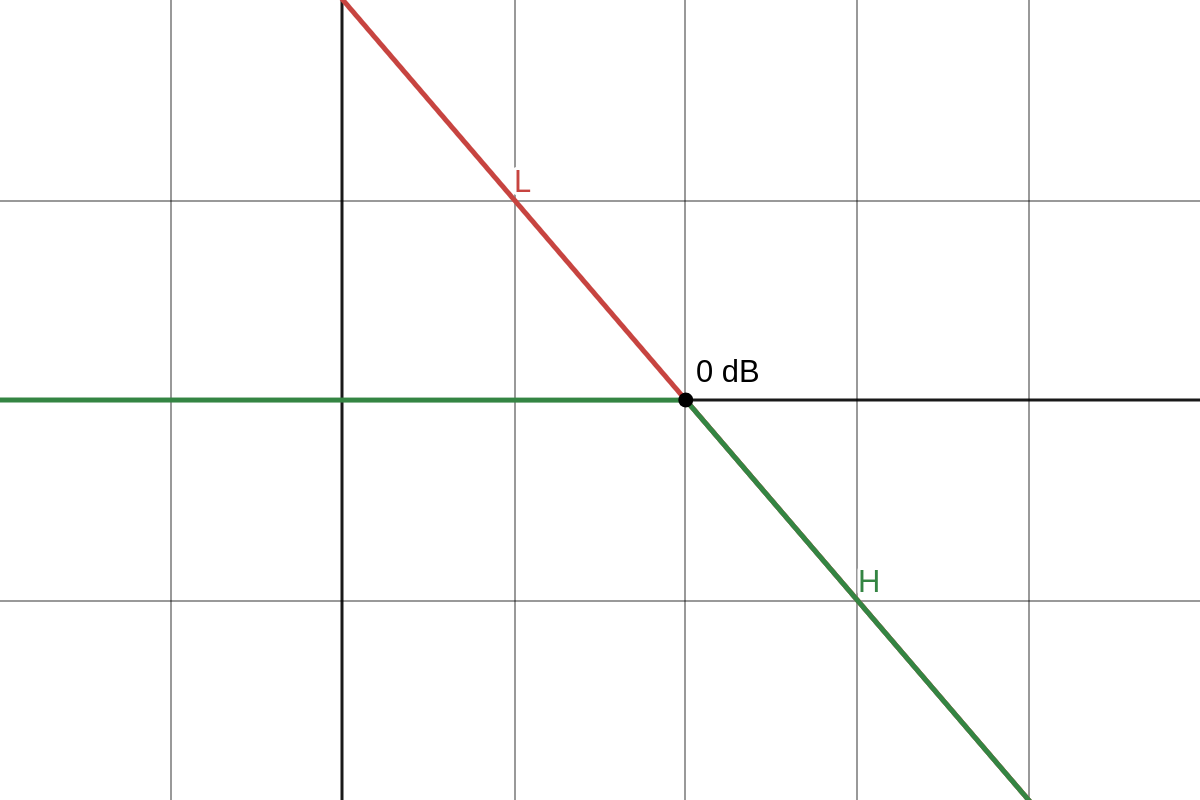
\includegraphics[scale=0.28]{../figures/lh.png}
	\end{center}

\end{minipage}

\par\bigskip

La media frequenza, cioè il punto dove la $H(j\omega)$ smette di tracciare gli 0 dB e inizia a seguire la $L(j\omega)$, sarà quindi $|L(j\omega)| \sim 1$.

\par\smallskip

Possiamo definire poi le regole empiriche sul il margine di fase:
\begin{itemize}
	\item $M_\phi > 75^\circ$ il sistema si comporta come un sistema del primo ordine;
	\item $M_\phi \leq 75^\circ$ il sistema si comporta come il sistema un secondo ordine.
\end{itemize}

Un'interpretazione intuitiva può essere che, se il margine di fase è alto, allora il sistema è molto stabile e quindi dimostrerà maggior comportamento del primo ordine, mentre viceversa se il margine di fase è basso, il sistema sarà sempre più vicino alla pura oscillazione, e quindi dimostrerà comportamento del secondo ordine.

Possiamo quindi riassumere di aver fatto le seguenti considerazioni sulla funzione di trasferimento in ciclo chiuso:
\begin{itemize}
	\item Il sistema in ciclo chiuso ha un comportamento di tipo passa basso;
	\item $H(j\omega)$ è caratterizzata da un polo dominante reale se $M_\phi > 75^\circ$, o da una coppia di poli dominanti complessi coniugati se $M_\phi \leq 75^\circ$;
	\item La \textbf{pulsazione di rottura} (nel caso di sistemi approssimabili al prim'ordine) o \textbf{pulsazione naturale} (secondo ordine) sono approssimate dalla pulsazione di taglio a 0 dB della funzione di anello $L$ (generalmente detta \textbf{pulsazione critica});
	\item La pulsazione critica è anche un'approssimazione (per difetto se $M_\phi < 90^\circ$, per eccesso altrimenti) della banda passante del sistema in ciclo chiuso;
	\item Lo smorzamento del sistema in ciclo chiuso è approssimato da:
		$$
		\xi \approx \frac{M_\phi}{100}, \quad M_\phi \leq 75^\circ
		$$
\end{itemize}

\subsection{Specifiche controllore}
Ricordiamo quindi che del controllore abbiamo le specifiche:
\begin{itemize}
	\item \textbf{Statiche};
	\item \textbf{Dinamiche};
	\item \textbf{Robustezza}, cioè \textit{stabilità robusta} (margini di fase e ampiezza, spesso indicati come diseguaglianze).
\end{itemize}

Il progetto del controllore si svolge seguendo una procedura \textit{Trial-and-error} (guidata), cioè per tentativi informati verso la soluzione localmente ottima (o una che la approssima).

\subsection{Specifiche statiche}
Per quanto riguarda le specifiche statiche ricordiamo che queste riguardano:
\begin{itemize}
	\item Stabilità;
	\item Frequenza di taglio e banda passante: qui si hanno particolari difficoltà per i sistemi a fase non minima;
	\item Verifica di specifiche statiche (errore a regime): in questo caso dobbiamo ricordare che per i diversi tipi di sistemi vale:
		\begin{itemize}
			\item Sistema di \textbf{tipo 0}, si ha l'errore a regime: 
				$$e(t\rightarrow\infty) = \frac{1}{1 + C(0)G(0)} = \frac{1}{1 + K_0}, \quad K_0 = C(0) G(0)$$
			\item Sistema di \textbf{tipo 1}, si ha l'errore a regime: $$e(t\rightarrow\infty) = \frac{1}{1 + \frac{C(0)G(0)}{s}} \Big|_{s\rightarrow 0} = 0$$
		\end{itemize}
		che si generalizzava col principio del modello interno.
\end{itemize}

Questo ci porta a definire due tipi di \textit{zone proibite}, cioè zone dove non vogliamo che passi il diagramma di Bode del modulo di $L(s)$:
\begin{itemize}
	\item Per sistemi di tipo 0, abbimo che $|L(s)|$ deve stare sopra una certa soglia alle basse frequenze;
	\item Per sistemi di tipo 1 si ha una situazione simile, dove la zona proibita ha però un aspetto più simile ad un trapezio:
\end{itemize}

\noindent
\begin{minipage}{\textwidth}

	Complessivamente, sul grafico le zone hanno il seguente aspetto:
	\begin{center}
		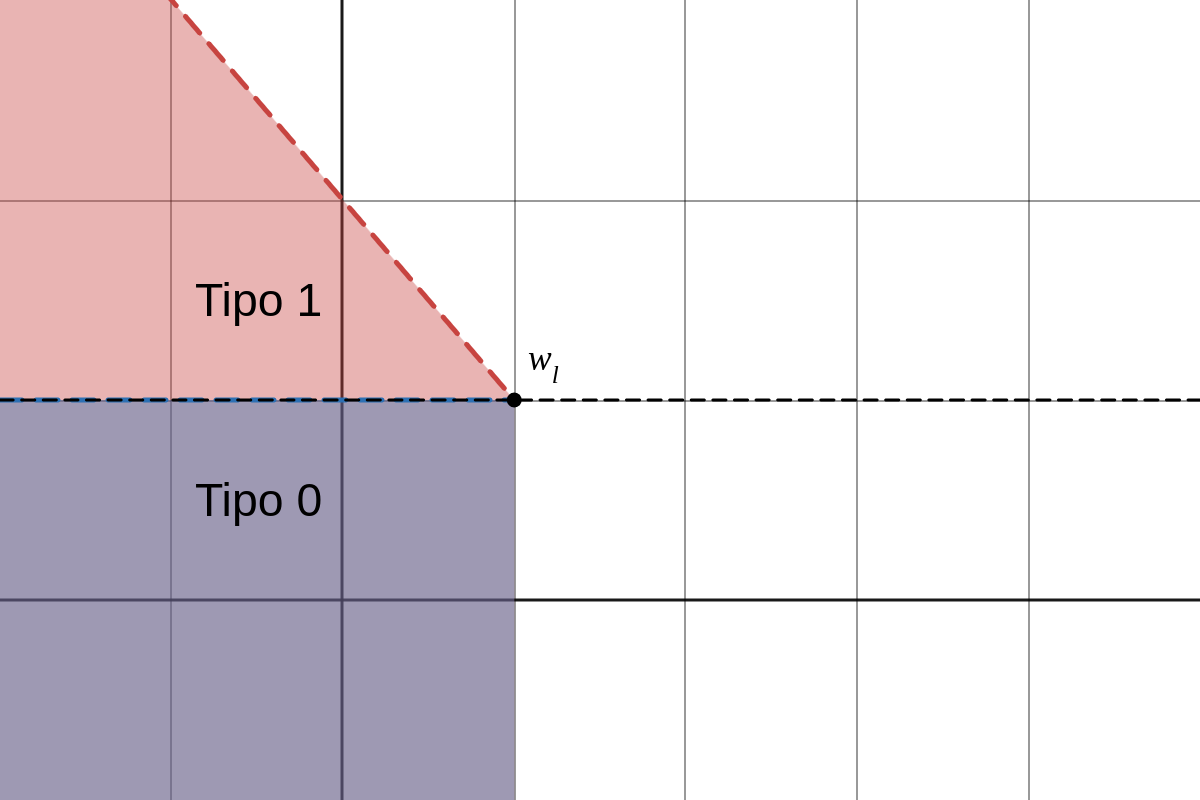
\includegraphics[scale=0.28]{../figures/loop_shaping_lower.png}
	\end{center}

\end{minipage}

\subsubsection{Rumori statici}
Una nota sui disturbi può farsi anche qui, in relazione agli \textit{attuatori}: potremo infatti considerare controllori dati da coppie $C(s)$ $A(s)$, controllore-atuoatore, col loro disturbo.
Questo disturbo, che si va a porre effettivamente come quello del primo sistema visto in 25.2.3, modelliza le imprecisioni dell'attuatore stesso.

In ogni caso, noi accenneremo soltanto, ma non useremo, questo modello.

\subsubsection{Rumori di misura}
Ricordiamo anche l'esistenza dei rumori di misura $N(s)$, diversi dai disturbi di carico o dai segnali di riferimento solitamente per l'alta frequenza.
Anche per questo motivo vogliamo attenuare il più possibile i segnali in alta frequenza.

\noindent
\begin{minipage}{\textwidth}

	Questo ci porta alla formazione di un'altra \textit{zona proibita}, alle alte frequenze al di sopra di un fattore di attenuazione in alta frequenza:
	\begin{center}
		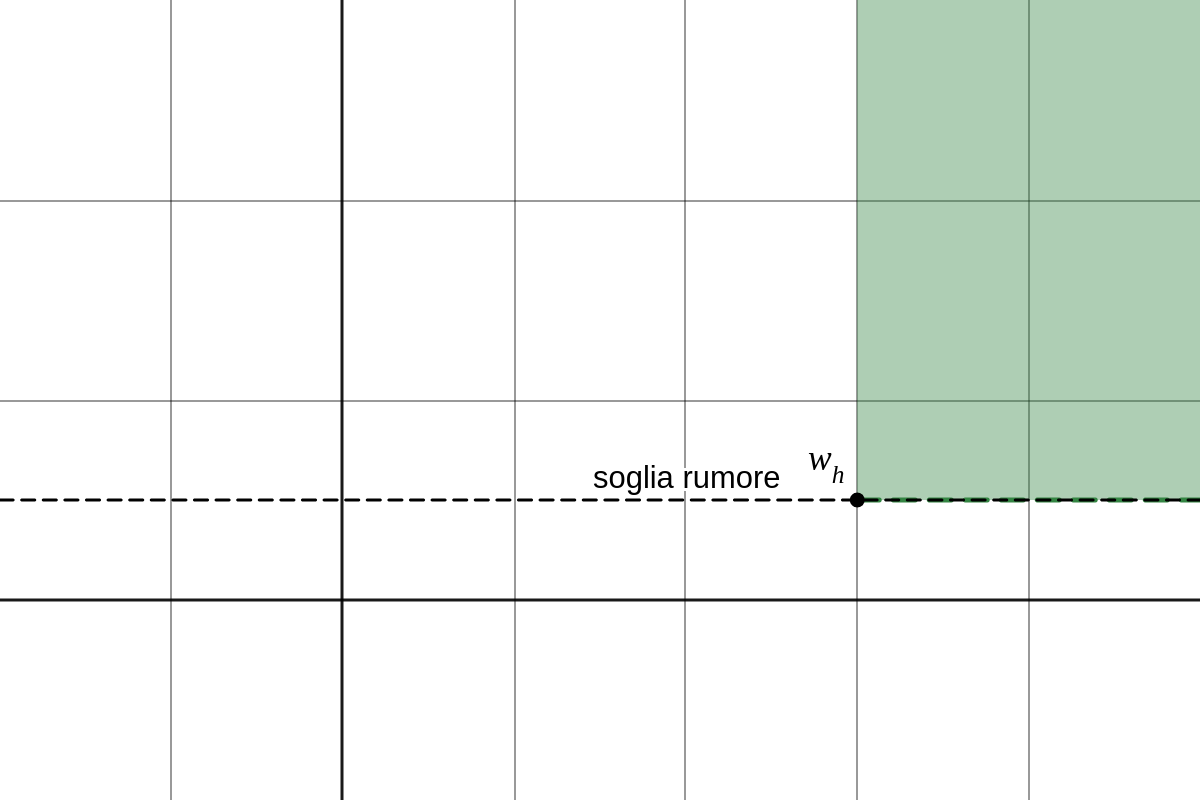
\includegraphics[scale=0.28]{../figures/loop_shaping_higher.png}
	\end{center}

\end{minipage}

\subsubsection{Zone proibite}
Avremo quindi definito sul diagramma del modulo della funzione di anello $L(s) = C(s) G(s)$ le cosiddette \textbf{zone proibite}, che potremo individuare come:
\begin{center}
	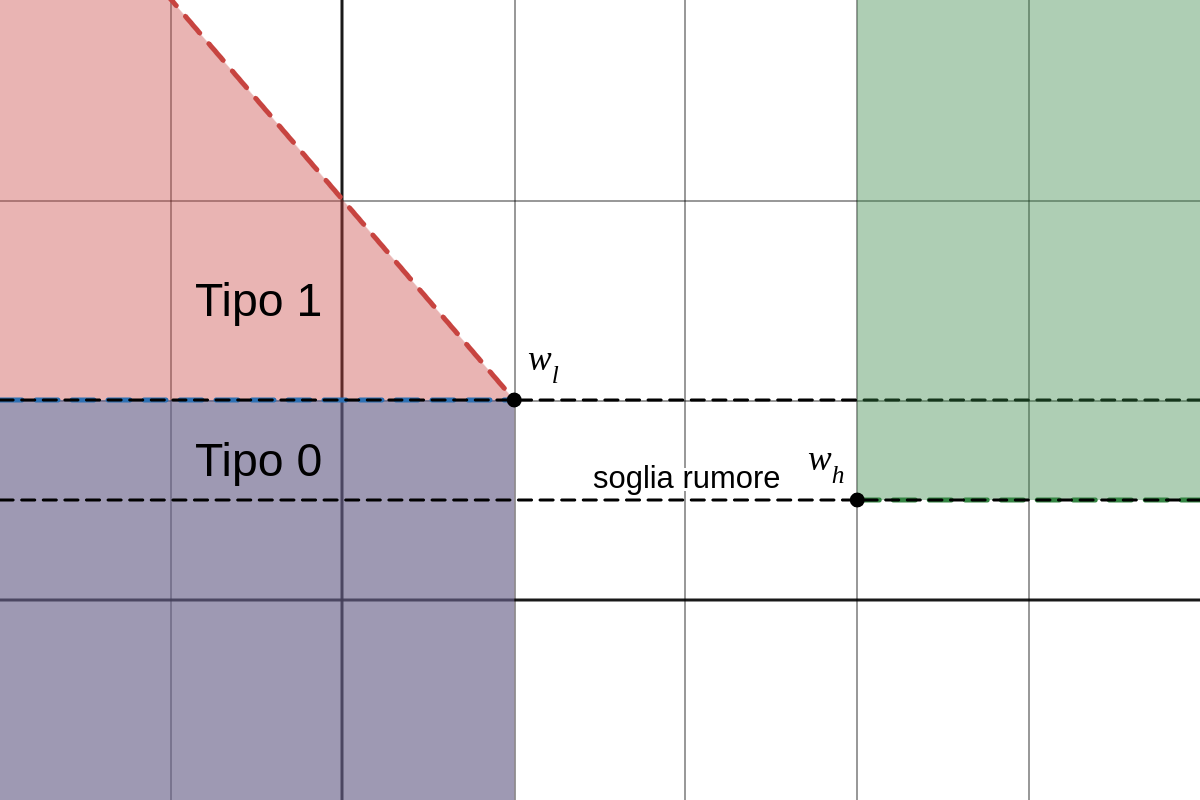
\includegraphics[scale=0.28]{../figures/loop_shaping_full.png}
\end{center}

Le zone proibite ci danno effettivamente la prima regione da individuare per effettuare il loop shaping.
Le specifiche di progetto dovranno quindi essere:
\begin{itemize}
	\item Tradotte in requisiti sul diagramma di Bode della funzione in anello;
	\item Rappresentate graficamente come regioni ammissibili del modulo della funzione di anello.
\end{itemize}

Il regolatore viene quindi progettato per "modellare" la funzione di anello all'interno delle regioni ammissibili.

\subsection{Specifiche dinamiche}
Per le specifiche dinamiche consideriamo:
\begin{itemize}
	\item Overshoot (\textit{sovraelongazione});
	\item Tempo di assestamento.
\end{itemize}

Sarà utile nella loro valutazione considerare la relazione globale:
$$
\xi \omega_0 \geq \frac{3}{t_{ass}}
$$

Ci tornerà poi utile il luogo delle radici, in quanto ricordiamo dalle regioni di vincolo viste in 20.1.3, che su questo possiamo piazzare agevolmente le specifiche di smorzamento, tempo di assestamento e pulsazione.

\begin{itemize}
	\item 
		In particolare, per il tempo di assestamento $T_{ass}$ ci interesserà prendere la regione da $-\xi\omega$ a $-\infty$ del luogo delle radici:
		\begin{center}
			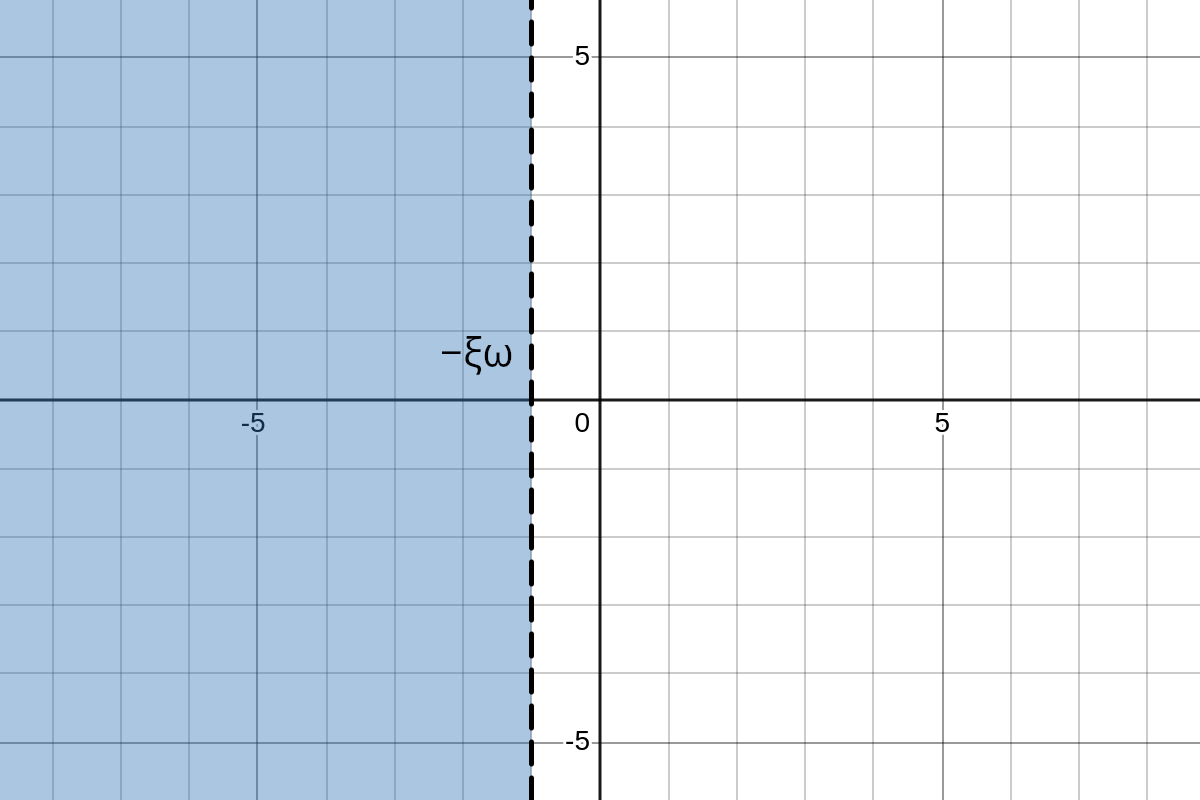
\includegraphics[scale=0.28]{../figures/fixed_time_region_cont.png}
		\end{center}

		\newpage

	\item Per l'overshoot potremmo tracciare le righe a smorzamento costante, in particolare con angolo $\beta = \sin^{-1} (\xi) $:
		\begin{center}
			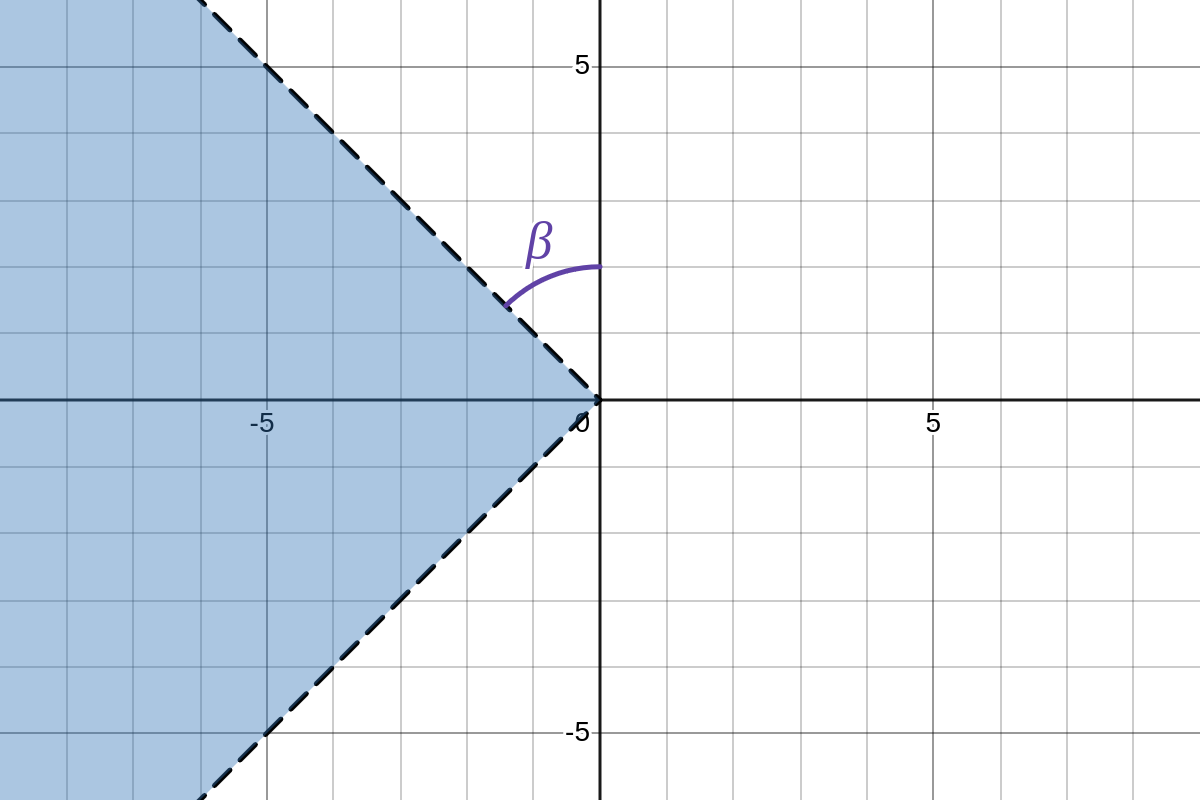
\includegraphics[scale=0.28]{../figures/fixed_damping_region_cont.png}
		\end{center}

		Ricordiamo poi che la sovraelongazione percentuale è definita come:
		$$
		S(\%) = e^{ \frac{-\xi \pi}{\sqrt{1 - \xi^2}} }
		$$

		Possiamo tracciare questa relazione su un grafico, con lo smorzamento $\xi$ alle ascisse e la percentuale di overshoot relativa alle ordinate:
		\begin{center}
			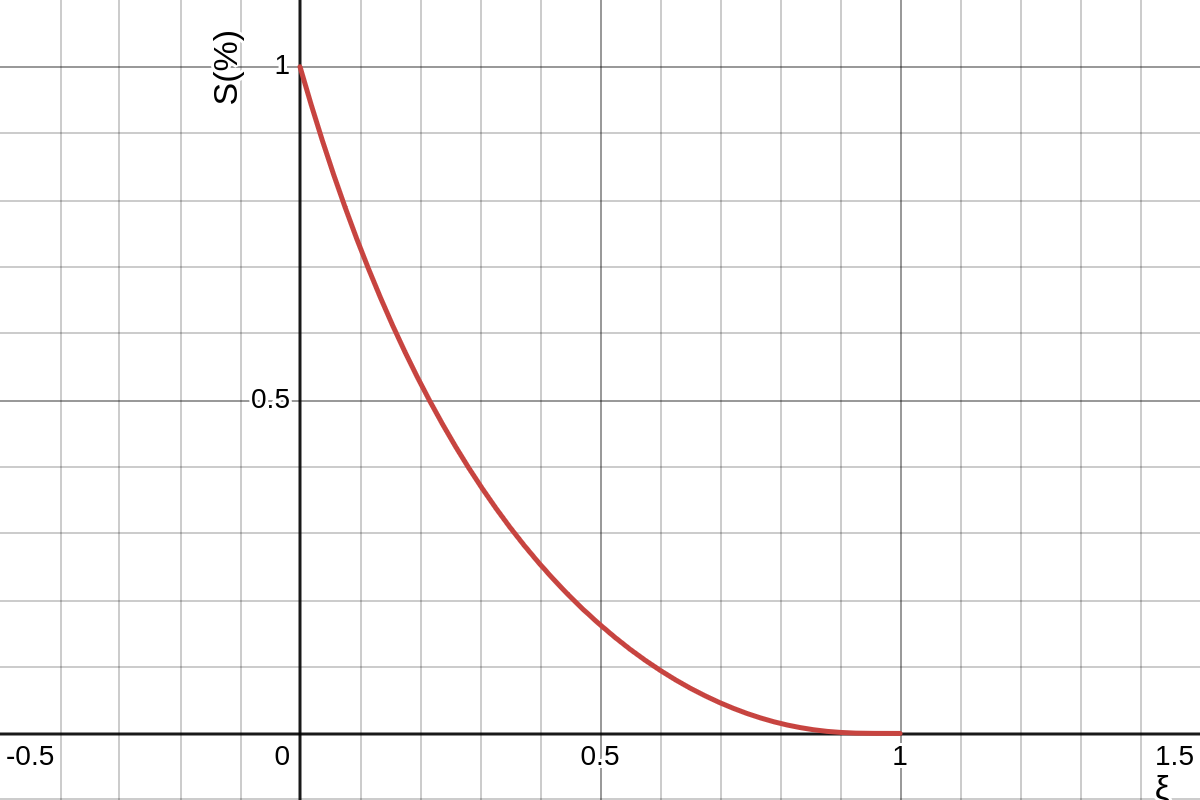
\includegraphics[scale=0.28]{../figures/damping_overshoot.png}
		\end{center}
		da cui si nota che esiste una relazione simile alla proporzionalità inversa fra le due grandezze.ds
\end{itemize}

Potremo quindi ottenere la zona ammissibile per i poli in catena chiusa tracciando la zona di validità che rispetta tutte le condizioni imposte.

\noindent
\begin{minipage}{\textwidth}

Ad esempio, combinando i due grafici sopra, otteniamo la zona di validità:

\begin{center}
	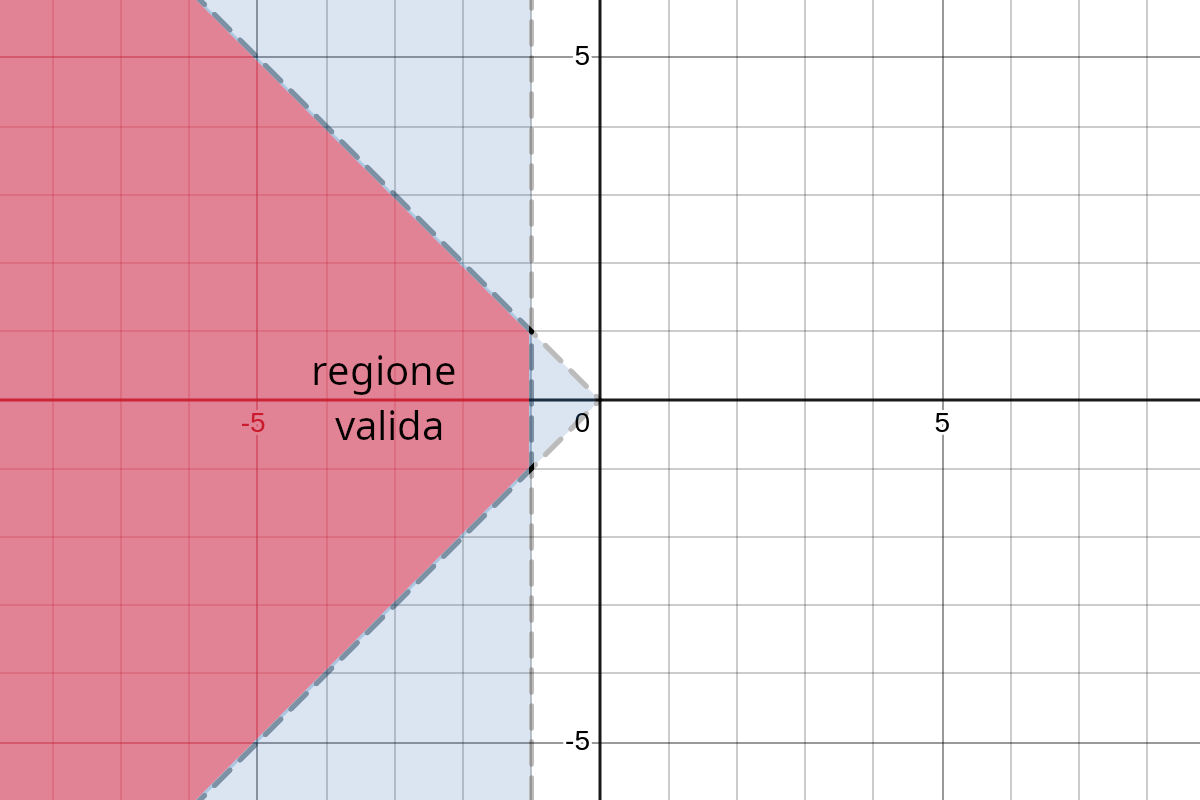
\includegraphics[scale=0.28]{../figures/valid_rlocus_region.png}
\end{center}

\end{minipage}

\subsubsection{Margini di fase e smorzamento}
Riguardo ai margini di fase, abbiamo che idealmente vorremmo $M_\phi$ di circa $90^\circ$ (come un integratore).
Questo potrebbe essere difficile da ottenere e si usa la regola empirica:
$$
M_\phi \geq M_\phi^* \approx 100 \xi^*
$$
in gradi, dove $\xi^*$ è il valore legato all'overshoot desiderato. # trova questa formula se hai voglia

\begin{itemize}
	\item Di base, una richiesta di overshoot uguale a 0 con margine di fase $M_\phi > 75^\circ$ indica di usare un'approssimazione del prim'ordine in catena chiusa (poli reali).
	\item Altrimenti, cioè quando si richiede $M_\phi \leq 75^\circ$, potrebbe essere necessaria un'approssimazione a poli dominanti:
		$$
		H(s) = \frac{1}{1 + \frac{2\xi}{\omega_0} s + \frac{s^2}{\omega_0^2}}
		$$
\end{itemize}

\subsubsection{Cancellazione poli/zeri}
Una tecnica che possiamo adottare, alla base dell'\textit{Internal Model Control}, è quella di scegliere:
$$
C'(s) = G^{-1}(s)
$$
e quindi di modellare il comportamento desiderato con un controllore $C''(s)$, che rispetta effettivamente le specifiche richieste.
Il controllore completo sarà a questo punto dato da:
$$
C_{tot}(s) = C'(s) \cdot C''(s)
$$

Chiaramente bisogna essere sicuri di non effettuare \textbf{cancellazioni improprie}, cioè di poli a parte reale maggiore o uguale a zero.
Questo potrebbe avere significato matematicamente, ma per l'inerente imperfezione dei sistemi reali, risulterebbe nella pratica in sistemi irrimediabilmente instabili.

\subsubsection{Esempio: loop shaping}
Prendiamo ad esempio la funzione di trasferimento:
$$
G(s) = \frac{\gamma}{m} \frac{1}{s + \frac{\beta}{m}} = 10 \frac{1}{s + 0.1}
$$ # dovrebbe essere il vecchio esempio sulla velocità di crocera

Non consideriamo disturbi.
Poniamo quindi che le specifiche date saranno:
\begin{itemize}
	\item Errore nullo in risposta al gradino, errore $< 5\%$ in risposta alla rampa;
	\item Nessuna sovraelongazione, tempo di assestamento al 95\% in risposta al gradino $< 15$ s.
\end{itemize}

La metodologia che adotteremo sarà:
\begin{itemize}
	\item Traduzione delle specifiche in requisiti sulla risposta armonica della funzione di anello;
	\item Progetto del regolatore $R$ in modo che $L = CG$ funzone di anello soddisfi i requisiti richiesti.
\end{itemize}

Vediamo quindi le specifiche una per una:
\begin{itemize}
\item Errore nullo in risposta al gradino: significa che dovremo usare un sistema di tipo 1 (cioè regolatore con un polo all'origine);
\item Errore $< 5\%$ in risposta alla rampa: significa che dovremo avere un guadagno in velocità $> 20$ (26 dB).
	Questo si ottiene valutando:
	$$
	e_{ss} = \lim_{t \rightarrow \infty} e(t) = \lim_{s \rightarrow 0} s \frac{1}{1 + G(s)} \cdot \frac{1}{s^2} = \frac{1}{s + s G(s)}
	$$
	posto:
	$$
	k_v = \lim_{s \rightarrow 0} s G(s)
	$$
	avremo che:
	$$
	e_{ss} = \lim_{s \rightarrow 0} \frac{1}{s + s G(s)} = \frac{1}{k_v}
	$$
	con $e_{ss} = 0.05$ (5 \%), si ha:
	$$
	k_v = \frac{1}{0.05} = 20
	$$
\item Nessuna sovraelongazione: significa che avremo un polo dominante reale, ovvero un margine di fase di almeno $75^\circ$;
\item Tempo di assestamento al 95 \% $< 15$ s: significa che la pulsazione critica sarà $> 0.2$ rad/s.

	Questo perché: dalla formula in 27.4 si ha:
	$$
	t_{ass} \geq \frac{3}{\xi \omega_0} \implies \omega_0 \geq \frac{3}{\xi t_{ass}} = 0.2
	$$
\end{itemize}

Vediamo quindi di aver individuato le zone proibite sul diagramma di modulo:

# grafico modulo

e di dover mantenere, per quanto riguarda la fase, il margine di fase:

# grafico fase

\par\smallskip

Una possibilile soluzione, a questo punto, sarà quella di sfruttare il controllore:
$$
C(s) = \frac{s + 0.5}{s}
$$
che aggiunge uno zero per alzare la fase della pulsazione critica.

In questo caso si otterranno i diagrammi di modulo e fase:

# grafici modulo e fase corretti

\subsubsection{Reiezione dei disturbi di carico}

Reintroduciamo quindi i disturbi, ricordando le funzioni di sensitività introdotte in 26.1.4:
$$
Y(s) = \frac{1}{1 + C(s)G(s)}D(s) = \frac{1}{1 + L(s)} D(s)
$$

Ricordiamo in particolare di aver definito le funzioni di sensitività e sensitività \textit{complementare}:
$$
S(s) = \frac{1}{1 + L(s)}, \quad H(s) = \frac{L(s)}{1 + L(s)}
$$
e facciamo l'osservazione fondamentale che:
$$
S(s) + H(s) = \frac{1}{1 + L(s)} + \frac{L(s)}{1 + L(s)} = 1
$$

Non è possibile ottenere robustezza ai disturbi di carico alle frequenze in cui la funzione di sensitività complementare $H(s)$ è piccola.
Nel nostro caso, $H(s)$ è piccola alle alte frequenze, quindi in quella regione avremo una cattiva reiezione dei disturbi di carico.
Questo non ci disturba in quanto i disturbi di carico sono situati solitamente nelle basse frequenze.

Vorremo quindi riportare il vincolo sui disturbi di carico a un vincolo sulla funzione di anello.
Prendiamo quindi:
$$
|S(j\omega)| \leq \epsilon_n, \quad \omega \in [0, \omega_n]
$$
dove $\omega \in [0, \omega_n]$ rapppresenta le basse frequenze.

Prendiamo quindi: 
$$
|S(j\omega)| \leq \epsilon_n \implies |1 + L(j\omega)| \geq \frac{1}{\epsilon_n}
$$
che potremo approssimare a:
$$
|L(j\omega)| \geq \frac{1}{\epsilon_n}
$$

\subsubsection{Reiezione dei rumori di misura}
Reintroduciamo anche i rumori di misura, come visti sempre nella 26.1.4:
$$
Y(s) = \frac{C(s)G(s)}{1 + C(s) G(s)} N(s) = \frac{L(s)}{1 + L(s)} N(s)
$$

Qui valgono essenzialmente le considerazioni fatte sui disturbi di carico, ma al contrario: si richiede che, visto che la funzione di trasferimento fra rumore di misura ed uscita è la sensitività complemntare, questa sia circa 1 a regime (basse frequenze) per soddisfare gli obiettivi di controllo.
Fondamentalmente, non potremmo alta precisione con rumori di precisione alle basse frequenze.
Anche questo non ci disturba in quanto il rumore di misura sta fondamentalmente nelle alte frequenze.

Vorremo quindi riportare anche questo ad un vincolo sulla funzione di anello, prendendo:
$$
|H(j\omega)| \leq \epsilon_n, \quad \omega \in [\omega_n, +\infty]
$$
dove $\omega \in [\omega_n, +\infty]$ rappresenta le alte frequenze.
Prendiamo quindi:
$$
|H(j\omega)| \leq \epsilon_n \implies \frac{|L(j\omega)|}{|1 + L(j\omega)|} \leq \epsilon_n
$$
che potremo approssimare a:
$$
|L(j\omega)| \leq \epsilon_n
$$


\end{document}
